The five reductions of Table~\ref{tab:versions_names} are compared on the same exposures in
Table~\ref{tab:versions}. Improved v2 and v3 run in \banzai{} from the raw frames; improved v1 is the set of
corrections applied to the archive products. Improved v3 is the final version (Chapter~\ref{sec:sites}). Instead of
refitting the arcs after the reduction, as v1 does, it uses the 1.1.0 arc fit with the added arc lines
(Section~\ref{sec:sites_arcs}), followed by the telluric zero point. Our \banzai{}~1.1.0 run already applies that zero
point, because the stage was already in our copy of the code when the run was made
(Table~\ref{tab:versions_names}). The two runs therefore do not differ in this respect, and the zero point does not
affect any other row of the table.

\begin{table}[!htbp]
\centering
\caption{The same exposures in the five reductions (Fairall~9: the 50 exposures with archive products; EG\,21: 18;
Feige\,110: 39, from raw only). Fringe metric as in Table~\ref{tab:summary}; per-spectrum residual: rms of each red-order spectrum about a fitted
power law (Fig.~\ref{fig:versions_individual}); small-scale scatter between spectra in per cent; [O\,{\sc iii}]
scatters are robust rms in per cent. 6500--7500\,\AA{} and water-band rows: per-spectrum rms of the 12/150\,\AA{}
high-pass (see Conventions) in the clean windows 6620--6850, 6960--7150 and 7350--7550\,\AA, or inside the band
(Fig.~\ref{fig:zoom}). For Fairall~9 the 6500--7500\,\AA{} row gives only the frame-specific part: the median over all
spectra is removed first, which removes the galaxy's narrow lines and anything common to all frames. In Feige\,110, 1.1.0 is low by
construction (each standard is divided by its own observed/expected ratio over most of the red order).}
\label{tab:versions}
\small
\begin{tabular}{lccccc}
\toprule
 & \banzai{}~1.0.1 & \banzai{}~1.1.0 & \multicolumn{3}{c}{improved} \\
Metric & (archive) & (stock) & v1 & v2 & v3 \\
 & (\%) & (\%) & (\%) & (\%) & (\%) \\
\midrule
\multicolumn{6}{l}{\textit{Fairall~9}}\\
Red fringe metric & 13.7 & 8.1 & 2.6 & 2.1 & 1.9 \\
Per-spectrum residual from a power law & 16.9 & 11.2 & 4.9 & 3.7 & 3.4 \\
Blue small-scale scatter 3500--4000\,\AA & 1.61 & 1.32 & 1.44 & 1.37 & 1.33 \\
Blue small-scale scatter 4000--4600\,\AA & 1.84 & 1.49 & 1.64 & 1.49 & 1.47 \\
Blue small-scale scatter 4600--5200\,\AA & 2.00 & 1.64 & 1.82 & 1.64 & 1.64 \\
Blue small-scale scatter 5200--5700\,\AA & 2.78 & 2.37 & 2.60 & 2.35 & 2.31 \\
Red small-scale scatter 5000--6000\,\AA & 2.08 & 0.99 & 1.09 & 0.96 & 0.95 \\
Red small-scale scatter 6000--6800\,\AA & 1.37 & 0.97 & 1.01 & 0.89 & 0.88 \\
Red small-scale scatter 7000--7500\,\AA & 3.18 & 1.94 & 1.65 & 1.63 & 1.35 \\
Red small-scale scatter 7700--8500\,\AA & 7.68 & 3.74 & 2.17 & 2.12 & 1.96 \\
Red small-scale scatter 8500--9500\,\AA & 12.74 & 6.11 & 3.68 & 3.55 & 3.85 \\
{[O\,{\sc iii}]} flux, blue order & 12.7 & 11.2 & 8.8 & 11.1 & 9.8 \\
{[O\,{\sc iii}]} flux, red order & 27.6 & 8.5 & 10.5 & 8.6 & 11.2 \\
Red/blue {[O\,{\sc iii}]} ratio & 29.2 & 8.9 & 9.7 & 8.5 & 6.9 \\
6500--7500\,\AA{} high-pass, frame-specific part & 2.52 & 1.23 & 1.17 & 0.98 & 0.93 \\
Water band 7170--7330\,\AA & 5.84 & 3.22 & 1.71 & 3.85 & 1.71 \\
Water band 8130--8360\,\AA & 16.10 & 7.95 & 3.17 & 4.03 & 3.21 \\
\midrule
\multicolumn{6}{l}{\textit{EG\,21}}\\
Red fringe metric & 9.3 & 2.7 & 2.1 & 1.6 & 1.5 \\
Per-spectrum residual from a power law & 11.7 & 4.0 & 4.2 & 3.0 & 2.5 \\
Red small-scale scatter 7000--7500\,\AA & 3.35 & 1.34 & 1.78 & 1.03 & 1.06 \\
Red small-scale scatter 7700--8500\,\AA & 9.02 & 2.43 & 2.46 & 1.85 & 1.71 \\
Red small-scale scatter 8500--9500\,\AA & 13.13 & 3.56 & 3.40 & 3.07 & 3.01 \\
6500--7500\,\AA{} high-pass & 3.01 & 1.14 & 2.90 & 1.10 & 0.88 \\
Water band 8130--8360\,\AA & 9.96 & 3.31 & 2.93 & 2.78 & 2.23 \\
\midrule
\multicolumn{6}{l}{\textit{Feige\,110 (flux / reference)}}\\
6500--7500\,\AA{} high-pass & -- & 0.68 & -- & 1.22 & 0.97 \\
7750--8900\,\AA & -- & 1.67 & -- & 3.01 & 2.00 \\
\bottomrule
\end{tabular}
\end{table}

Improved v3, run in one pass from the raw frames, has the best fringe correction of all reductions, without having
to undo any earlier processing. The red fringe metric of Fairall~9 is 1.9 per cent (\banzai{}~1.0.1
13.7, 1.1.0 8.1, improved v1 2.6, v2
2.1) and the residual of the individual spectra from a power law
3.4 per cent (Fig.~\ref{fig:versions_individual}). On EG\,21 it is the best in every red
metric but one (small-scale scatter at 7000--7500\,\AA: 1.06 against 1.03 per cent for v2). In the blue order and at 5000--6800\,\AA{} the runs from raw are better than both reductions based on the archive
products, because they have no destroyed pixels and the data are resampled only once. The red/blue [O\,{\sc iii}] ratio, the most
direct test of the relative calibration of the orders, scatters by 6.9 per cent (1.1.0
8.9, v1 9.7, v2 8.5). With the ensemble flux
calibration (Section~\ref{sec:flux_ensemble}) the blue [O\,{\sc iii}] flux scatters by 9.8 per
cent, against 11.2 for 1.1.0 and 11.1 for v2, which both use the single nearest
standard. Improved v1 reaches 8.8 per cent, with an ensemble of the whole campaign rather than of the nine nearest
standards. Inside the water bands v3 matches v1 at 7170--7330\,\AA{} (1.71 against
1.71 per cent) and at 8130--8360\,\AA{} (3.21 against
3.17). The water absorption still changes from night to night ($\approx3.5$ per
cent rms in the level of the 8110--8380\,\AA{} band), and a median of nine standards cannot follow this. The O$_2$ A band
(7580--7700\,\AA) is flagged in the science spectra of v3 (mask bit 2, Section~\ref{sec:flux_tell}).

Figure~\ref{fig:fringe_band} shows the effect of the fringe settings of v3 at 6000--7700\,\AA. In the 18 EG\,21
spectra, the rms of the high-passed spectra in the line- and telluric-free windows drops from 3.91 per cent
(uncorrected) and 0.99 per cent (initial configuration of the pipeline's fringe model) to 0.94 per cent. In all 100
Fairall~9 spectra of the v3 run, the frame-specific part drops from 1.36 per cent (initial configuration) to
0.94 per cent; without any fringe correction it is 1.12 per cent.

Figure~\ref{fig:final_spectra} shows what this means for the spectra themselves: a typical epoch in
\banzai{}~1.0.1 and in improved v3, and the red order of all epochs side by side.

\begin{figure}[!htbp]
\centering
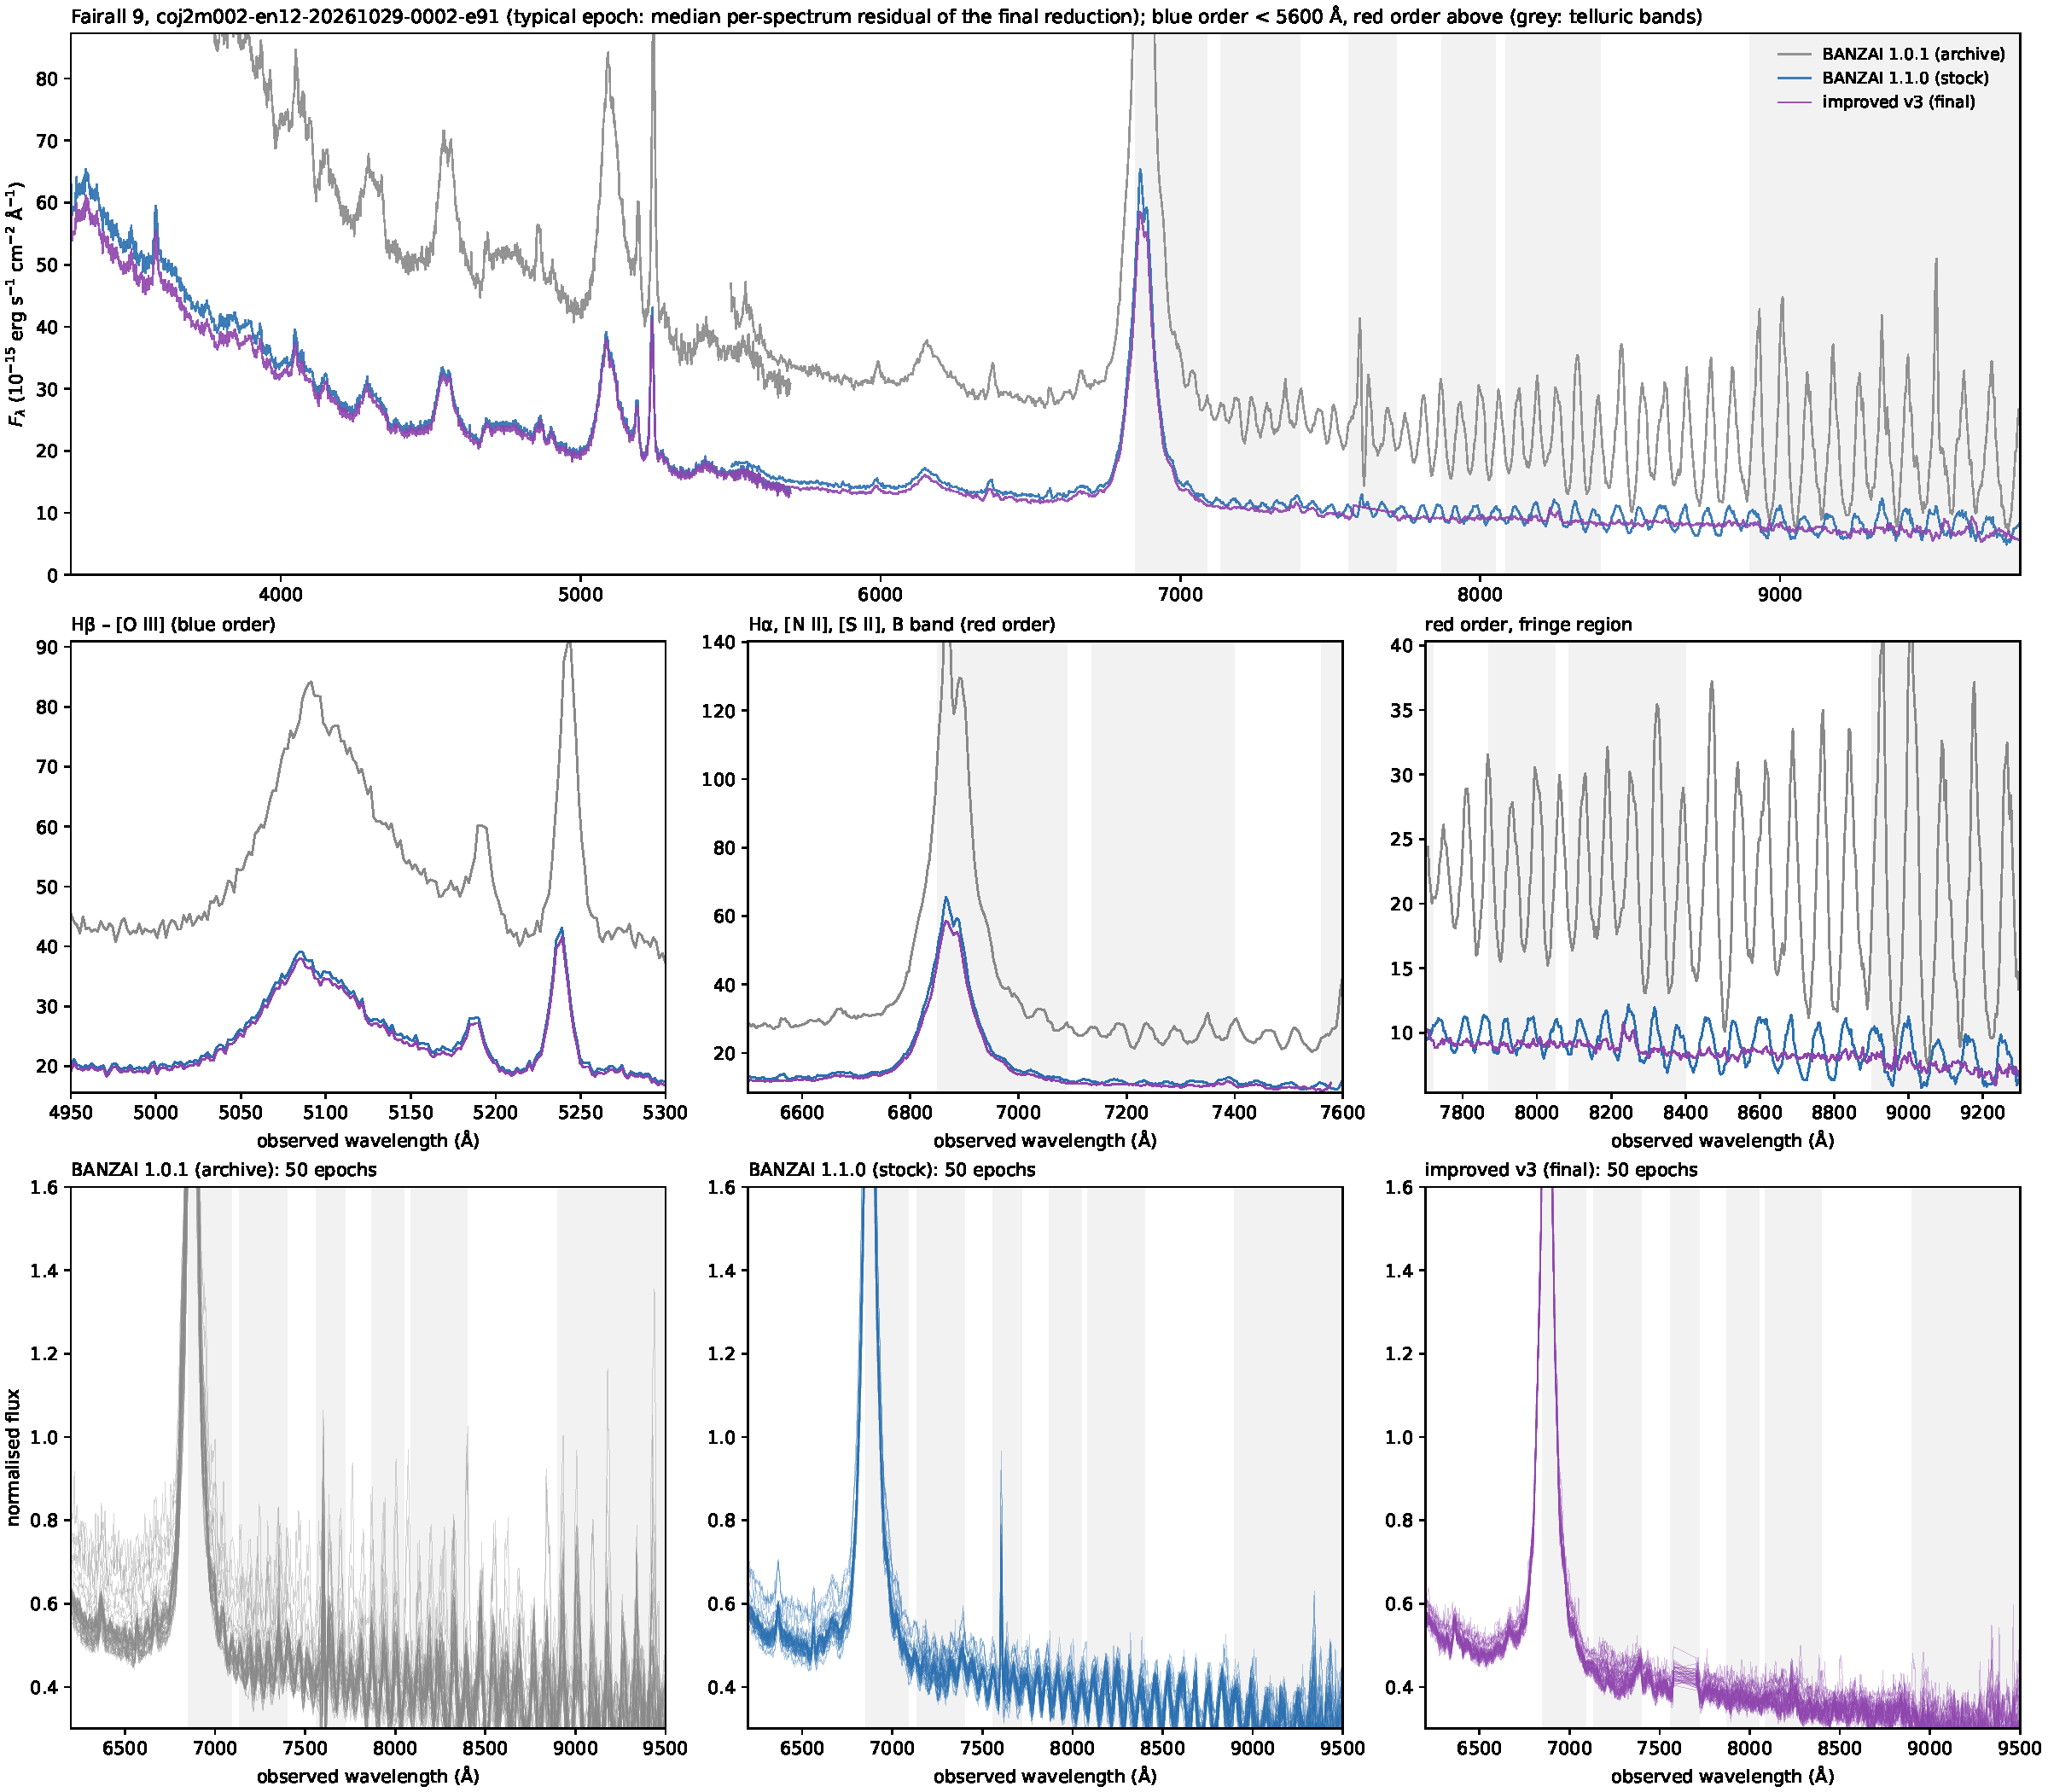
\includegraphics[width=\textwidth]{figures/fig_final_spectra.pdf}
\caption{Fairall~9 in the archive (\banzai{}~1.0.1, grey) and in the final reduction (improved v3, purple). Top: a
typical epoch (median per-spectrum residual of v3), both orders; the archive is multiplied by 0.44, the median ratio of
the two, because 1.0.1 does not divide by the exposure time (Section~\ref{sec:flux_banzai}). Middle: the red end of the
same epoch, where the archive carries the fringes. Bottom: the red order of all 50 epochs with archive products, each
divided by its flux at 5100--5200\,\AA{} (blue order); the spread is the AGN variability plus the calibration errors.
Grey bands: telluric absorption.}
\label{fig:final_spectra}
\end{figure}

\begin{figure}[!htbp]
\centering
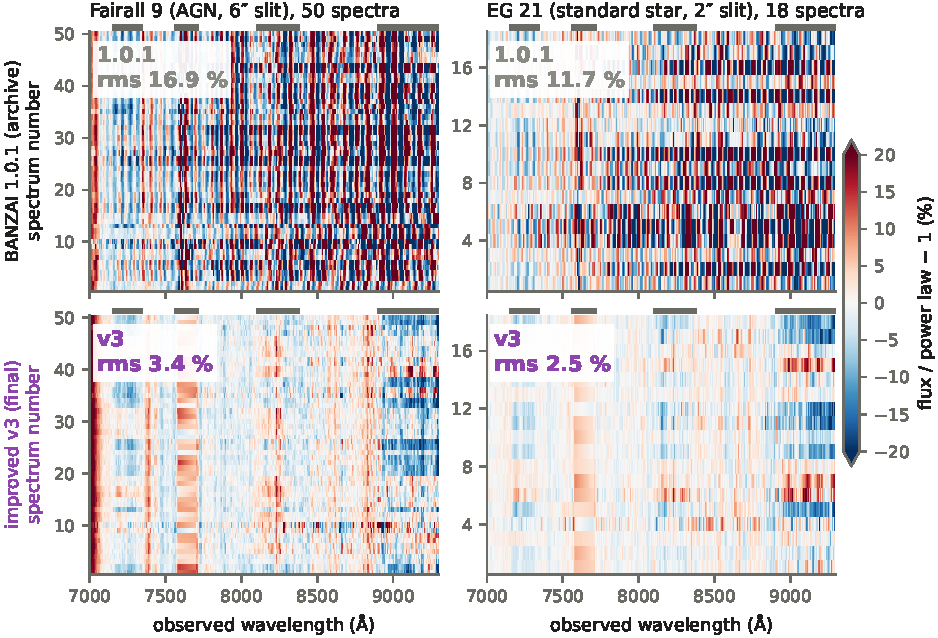
\includegraphics[width=\textwidth]{figures/fig_versions_individual.pdf}
\caption{Every red-order spectrum (one row each, in time order) divided by a power law fitted at 7000--9800\,\AA,
in the archive (\banzai{}~1.0.1, top) and in improved v3 (bottom); Fairall~9 left, EG\,21 right. The vertical stripes
in the archive are the fringes. The rms is the median over spectra in the clean windows 7750--8050 and
8450--8900\,\AA. Grey bars above each panel: telluric bands, left out of the fit. Cut at 9300\,\AA, beyond which the
night-to-night change of the water-vapour absorption dominates; 1.1.0 and v1 are in Table~\ref{tab:versions}.}
\label{fig:versions_individual}
\end{figure}

\begin{figure}[!htbp]
\centering
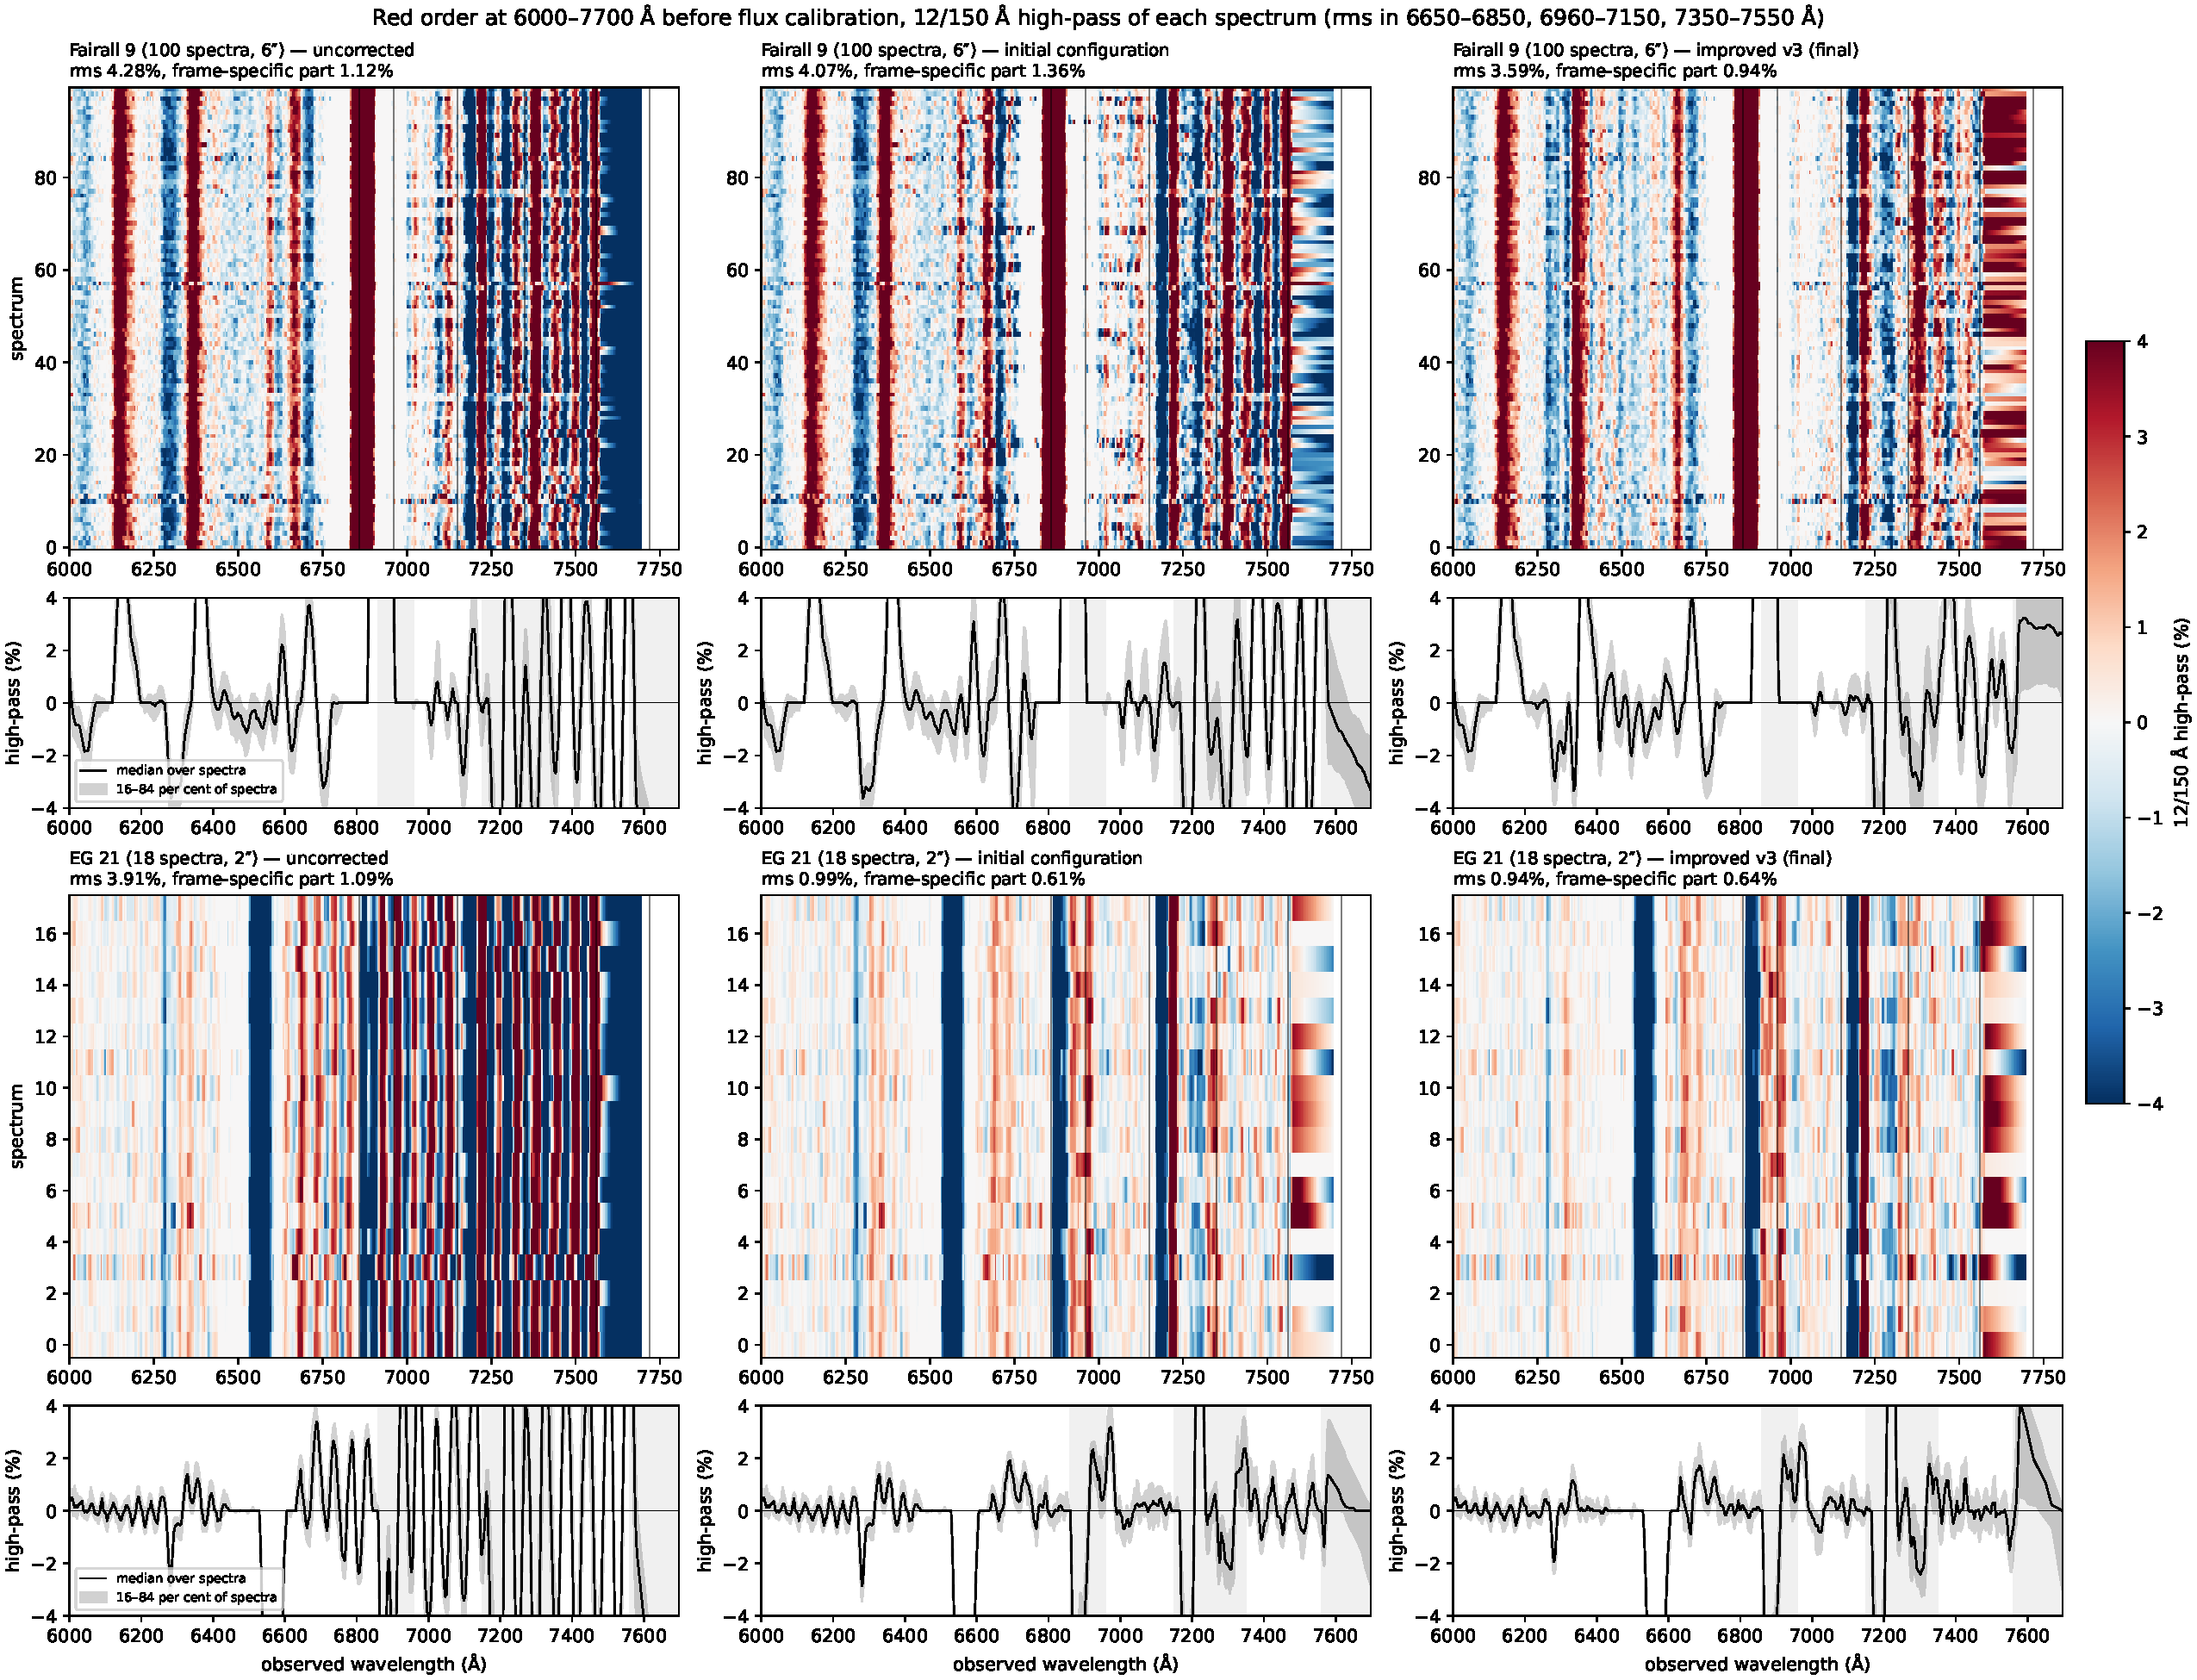
\includegraphics[width=\textwidth]{figures/fig_fringe_band.pdf}
\caption{Small-scale structure of the red order at 6000--7700\,\AA{} before flux calibration: rms of the
12/150\,\AA{} high-pass in the clean windows 6650--6850, 6960--7150 and 7350--7550\,\AA, median over spectra (18 of
EG\,21; all 100 of Fairall~9 in the v3 run, not only the 50 with archive products), for the uncorrected spectra, the
initial configuration of the harmonic fringe model in the pipeline, and improved v3
(Sections~\ref{sec:fringe_pipeline}--\ref{sec:fringe_joint}). For Fairall~9 the frame-specific part (the median over
all spectra removed) separates the fringes from the galaxy's narrow lines ([N\,{\sc ii}], [S\,{\sc ii}]), which the whole high-pass
includes.}
\label{fig:fringe_band}
\end{figure}

\begin{figure}[!htbp]
\centering
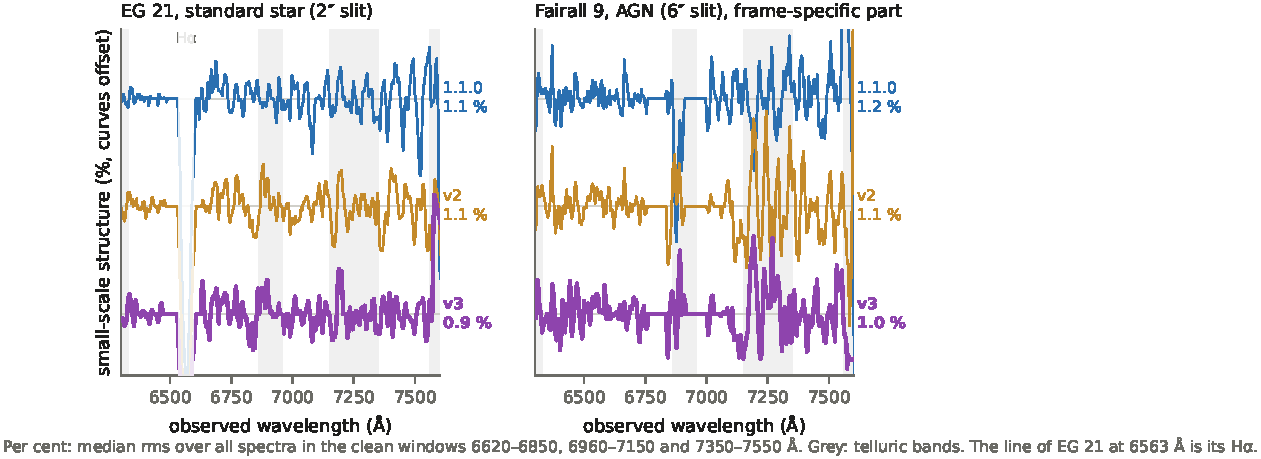
\includegraphics[width=\textwidth]{figures/fig_zoom_6300_7700.pdf}
\caption{Small-scale structure at 6300--7700\,\AA{} (12/150\,\AA{} high-pass of the flux-calibrated red order) in a
typical spectrum (the median rms of improved v3) of EG\,21 (left) and of Fairall~9 (right; the median over spectra
removed, since its narrow lines fall in these windows), for \banzai{}~1.1.0, improved v2 and improved v3, offset for
clarity. Beside each curve: the median rms over all spectra in the clean windows. In this band the three reductions
differ little (1.1 to 0.9 per cent); the fringing that the improved pipeline removes is mostly redward of 7700\,\AA{}
(Fig.~\ref{fig:versions_metrics}). Feige\,110, shown in earlier versions of this figure, is left out: as a flux
standard of these reductions it is flat by construction.}
\label{fig:zoom}
\end{figure}

\begin{figure}[!htbp]
\centering
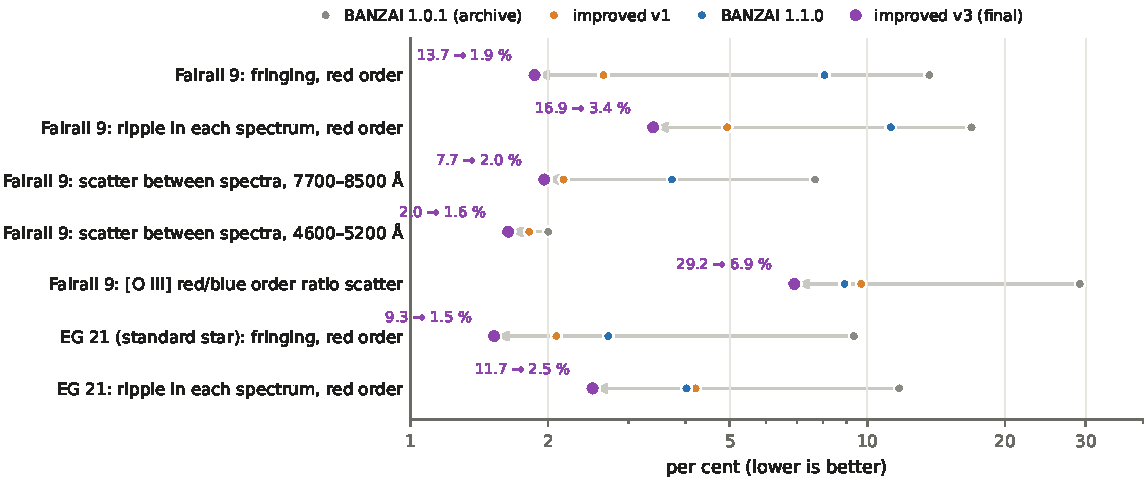
\includegraphics[width=\textwidth]{figures/fig_versions_metrics.pdf}
\caption{Summary of Table~\ref{tab:versions}: each row is one measure of quality (lower is better), each dot a
reduction, and the arrow runs from the archive (\banzai{}~1.0.1) to the final reduction (improved v3), whose values are
written above it. Fringing: the red-order fringe amplitude; ripple: the rms of each spectrum about a power law in the
clean windows of the red order; scatter: the small-scale scatter between the 50 Fairall~9 spectra.}
\label{fig:versions_metrics}
\end{figure}

